\documentclass[runningheads]{llncs}
% MICCAI 2026 (REG2026 challenge) submission. Springer LNCS format.
% Anonymized for double-blind review: no author names, affiliations, repo URLs, or grant IDs.
% Add the author block only at camera-ready.
% Class files (llncs.cls, splncs04.bst) are provided by the Overleaf LNCS template.
% Style: no LaTeX "--" or "---" (they render as en/em dashes); use single hyphens or rephrase.

\usepackage{graphicx}
\usepackage{booktabs}
\usepackage{amsmath}
\usepackage{amssymb}
\usepackage{xcolor}
\usepackage[hidelinks]{hyperref}

\begin{document}

\title{Grounded Ontology Walker: Interpretable Diagnostic Reasoning and Report Generation for Whole Slide Images}

\titlerunning{Grounded Ontology Walker}

\author{Anonymous}
\authorrunning{Anonymous}
\institute{Paper ID XXXX. Author information withheld for double-blind review.}

\maketitle

\begin{abstract}
Generating a pathology report from a whole-slide image (WSI) is increasingly framed as a reasoning problem:
a model should not only produce the report but also expose the diagnostic reasoning behind it. Free-form
generated reasoning is difficult to verify and can diverge from the reported findings. We present the
Grounded Ontology Walker (GOW), a discriminative pipeline in which the reasoning is an explicit walk over a
diagnostic ontology mined from expert reasoning chains, and the report is a deterministic render of that walk.
Every reasoning step is a valid ontology transition, so the chain is auditable, and because the report is
derived from the chain it is faithful to the reasoning by construction. Each diagnostic question is answered
from the specific image regions that a question-conditioned selector attends to, over patch features from
Virchow2, a frozen pathology foundation model, which grounds and localizes every decision. To remain safe on
organs that are absent from training, GOW includes a per-organ distribution-shift detector that flags unseen
organs and routes them through the nearest in-ontology topology with open-vocabulary naming, and we show it
generalizes to novel organs on public external slides. On the blind Test Phase 1 evaluation GOW attains an
overall score of 0.791: visual grounding is perfect (1.00, spanning background rejection, input sensitivity,
and cross-region consistency), the reasoning graph is recovered at edge F1 0.852 with matched-edge answer
similarity 0.772, and the report scores 0.572. On the development split held out from the training data,
reasoning-edge F1 is 0.922 and organ recognition 0.993. We report performance per metric and evaluation setting
and analyze the contribution of each component.

\keywords{Computational pathology \and Report generation \and Reasoning \and Multiple instance learning \and Out-of-distribution detection.}
\end{abstract}

\section{Introduction}
\label{sec:intro}
Automated report generation from whole-slide images (WSIs) is increasingly a joint task: produce a structured
pathology report together with the diagnostic reasoning that supports it, so the output is auditable. When the
reasoning comes from a free-form generator, however, individual steps are not guaranteed valid and the rationale
may be inconsistent with the reported findings.

This work targets the REG2026 (MICCAI 2026) challenge: given an H\&E WSI, a system produces an explicit reasoning
chain over a closed clinical question ontology plus a structured report (the workflow-reasoning interface) and
answers grounding questions on regions of interest (the visual-grounding interface), across seven organs. Expert
reasoning in the training data follows a bounded set of questions and transitions, defining a diagnostic ontology.

We formalize the reasoning as a traversal of this ontology, mined as a transition graph from the expert
reasoning chains. Inference is a deterministic walk over the graph, and the report is rendered deterministically
from the answers collected along the walk. We refer to the method as the Grounded Ontology Walker (GOW).

\noindent\textbf{Contributions.} (i)~The chain of thought is a deterministic walk over a transition graph mined
from expert chains, so every step is a valid, auditable ontology transition, not free-form text. (ii)~The report
is a deterministic render of the completed walk, faithful to the reasoning by construction. (iii)~A
question-conditioned pooler selects the patches that answer each question, scored against text embeddings of the
allowed responses, supporting open-vocabulary answering of rare classes. (iv)~A detector on the frozen features
flags organs absent from training and routes them safely. The critical path is discriminative and LLM-free,
hence reproducible and light enough for an offline single-GPU container.

\section{Related Work}
\label{sec:related}
\textbf{Report generation} typically couples a WSI encoder to a text decoder, increasingly a medical language or
multimodal model~\cite{geminimed,medgemma,openbiollm}, fluent but with little guarantee the findings are grounded
in tissue. \textbf{WSI foundation models}~\cite{virchow2,uni,provgigapath,hoptimus} give transferable patch
features and slide-level variants~\cite{prism,titan} summarize a slide; we use one tile encoder as a frozen
backbone and a vision-language model~\cite{conch} as a text-embedding space for answers. \textbf{Attention-based
MIL}~\cite{abmil,clam} aggregates patches with an interpretable attention map; we use a gated variant with a
question-conditioned pooler. \textbf{Structured-reasoning} methods encode clinical decisions as templates or
graphs; we instead mine the decision graph from data and make inference a deterministic walk inside a closed,
verifiable vocabulary.

\section{Methods}
\label{sec:method}
Figure~\ref{fig:pipeline} shows the full pipeline.

\begin{figure}[t]
\centering
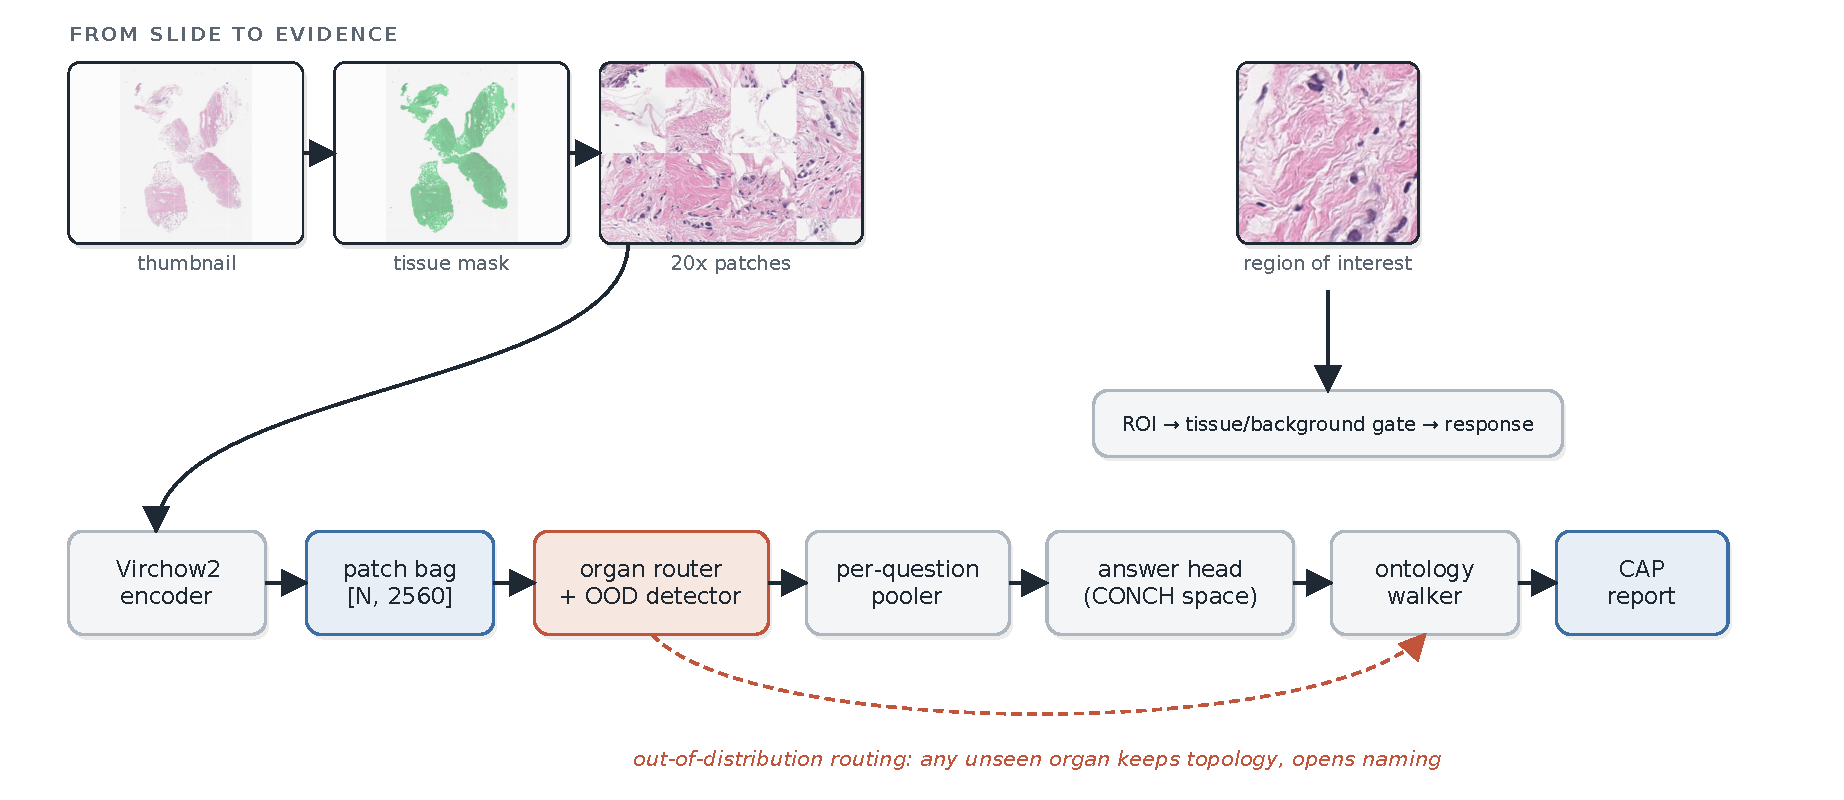
\includegraphics[width=0.82\textwidth]{figures/pipeline.pdf}
\caption{The Grounded Ontology Walker. Top: input stages on one slide (thumbnail, GrandQC tissue mask, 20x
patches, region of interest). Bottom: a frozen Virchow2 encoder embeds each patch into a bag; a gated-attention
MIL head predicts the organ and feeds the distribution-shift (OOD) detector; reasoning then proceeds question by
question, a question-conditioned pooler selecting patches, an answer head scoring them against text embeddings of
the allowed answers, and a mined transition table supplying the next question, until the walk is rendered into a
report. The dashed arrow routes an unseen organ through the nearest in-ontology topology.}
\label{fig:pipeline}
\end{figure}

\subsection{Tiling, encoding, and the slide bag}
Tissue is segmented with a quality-control model~\cite{grandqc} and the slide is tiled into 224-pixel patches
at 20x magnification, giving a variable-size bag of patches per slide. Each patch is embedded by the frozen
Virchow2~\cite{virchow2} foundation model into a 2560-dimensional vector formed by concatenating the class token
with the mean of the patch tokens. Because the encoder is frozen, the bag is precomputed once per slide and
reused by every downstream head. A slide thus yields a bag $H=\{\mathbf{h}_i\}_{i=1}^{N}$ with
$\mathbf{h}_i\in\mathbb{R}^{d}$, $d{=}2560$.

\subsection{Slide-level MIL: organ and global context}
A gated-attention MIL head~\cite{abmil} aggregates the bag into a slide vector and predicts the organ. With
$\boldsymbol{\phi}_i=\mathrm{ReLU}(\mathbf{W}\mathbf{h}_i+\mathbf{b})\in\mathbb{R}^{m}$ ($m{=}512$), the
attention weights and slide vector are
\begin{equation}
a_i=\frac{\exp\!\big(\mathbf{w}^{\!\top}(\tanh(\mathbf{V}\boldsymbol{\phi}_i)\odot\sigma(\mathbf{U}\boldsymbol{\phi}_i))\big)}
{\sum_j \exp\!\big(\mathbf{w}^{\!\top}(\tanh(\mathbf{V}\boldsymbol{\phi}_j)\odot\sigma(\mathbf{U}\boldsymbol{\phi}_j))\big)},
\qquad \mathbf{z}=\sum_i a_i\boldsymbol{\phi}_i ,
\end{equation}
and the organ posterior is $\mathbf{p}=\mathrm{softmax}(\mathbf{W}_o\mathbf{z})$; the gate lets a few informative
patches dominate $\mathbf{z}$. The bag mean $\bar{\mathbf{h}}=\tfrac1N\sum_i\mathbf{h}_i$ is the input to the distribution-shift
detector (Section~\ref{sec:ood}), and $\mathbf{p}$ conditions the answer heads on organ context.

\subsection{Per-question evidence selection}
\label{sec:qcp}
Reasoning proceeds one ontology question at a time. A question with CONCH text embedding $\mathbf{q}$ is
projected into the patch space, $\tilde{\mathbf{q}}=\mathbf{W}_q\mathbf{q}$, and each patch receives a
question-specific relevance $r_i=\mathrm{MLP}([\mathbf{h}_i;\tilde{\mathbf{q}}])$. The evidence combines a
soft-attention pool with a focal max-pool,
\begin{equation}
b_i=\mathrm{softmax}_i(r_i), \qquad
\mathbf{e}_q=\rho\!\Big(\underbrace{\textstyle\sum_i b_i\,\mathbf{h}_i}_{\text{soft pool}}
+\underbrace{\mathbf{h}_{\arg\max_i r_i}}_{\text{focal max}}\Big).
\end{equation}
The focal term matters clinically: a small but decisive focus (a microscopic tumor focus, a mitotic figure, a
granuloma) can determine the answer despite occupying a tiny fraction of the slide. Because $r_i$ is
question-conditioned, different questions attend to different patches, and $b_i$ localizes the tissue behind each
decision.

\subsection{Open-vocabulary answer heads}
Answers are scored in the text space of CONCH~\cite{conch}, a pathology vision-language model whose image-text
pretraining aligns morphology with terminology, so an answer is scored by the similarity of the evidence to its
text description and rare or unseen classes stay reachable. Let
$\mathcal{A}_q$ be the answers allowed at the current node, each with a CONCH text embedding $\mathbf{t}_a$. The
evidence, slide vector, and organ posterior are projected to a query
$\mathbf{g}=\pi([\mathbf{e}_q;\mathbf{z};\mathbf{p}])$, and answers are scored contrastively in the CLIP
sense~\cite{clip},
\begin{equation}
s(a)=\tau\,\frac{\mathbf{g}^{\!\top}\mathbf{t}_a}{\lVert\mathbf{g}\rVert\,\lVert\mathbf{t}_a\rVert},
\qquad \hat a=\arg\max_{a\in\mathcal{A}_q}s(a),
\end{equation}
with a learned temperature $\tau$. Restricting $\mathcal{A}_q$ to the node's allowed answers gives organ- and
context-masking for free and keeps every emitted string inside the ontology.

\subsection{Distribution-shift detection and safe routing}
\label{sec:ood}
The seven training organs are not an exhaustive list of the anatomy that can appear, so a slide may belong to an
organ the seven-way router cannot represent. We standardize the frozen bag mean and project it to a $k{=}128$ subspace,
$\mathbf{u}=\mathbf{P}\,(\bar{\mathbf{h}}-\boldsymbol{\mu})/\boldsymbol{\sigma}$. Rather than a single shared
covariance, we estimate a per-organ mean $\boldsymbol{\nu}_c$ and a ridge-regularized per-organ covariance
$\boldsymbol{\Sigma}_c$, and score a slide by its squared Mahalanobis distance to the nearest training
organ~\cite{mahalanobis},
\begin{equation}
D(\bar{\mathbf{h}})=\min_{c}\,(\mathbf{u}-\boldsymbol{\nu}_c)^{\!\top}\boldsymbol{\Sigma}_c^{-1}(\mathbf{u}-\boldsymbol{\nu}_c).
\end{equation}
The quadratic per-organ form is what lets the detector generalize to any of the seven routes rather than a
single one: leave-one-organ-out analysis (Section~\ref{sec:exp}) improves from $0.85$ to $0.98$ AUC when the
shared covariance is replaced by per-organ covariances. A slide routed to organ $c$ is flagged when
$D(\bar{\mathbf{h}})>\tau_c$, with $\tau_c$ fixed label-free from organ $c$'s in-distribution distances and scaled
for precision; a false flag on a seen organ costs more than a missed borderline novel organ, so only about $2\%$
of held-out in-distribution slides are flagged. A flagged slide walks the same routed topology, named by
open-vocabulary matching against the CAP library, so only the organ and diagnosis strings change, never the
reasoning edges.

\subsection{Training}
\label{sec:train}
The Virchow2 encoder is frozen; only the MIL, pooler, and answer heads are trained on the precomputed bags. The
organ head is supervised by cross-entropy and each answer node by a focal loss~\cite{focal} with $\gamma{=}1.5$
over its candidate set, combined as
\begin{equation}
\mathcal{L}=\lambda_o\,\mathrm{CE}(\mathbf{p},y_{\mathrm{org}})
+\frac{1}{|\mathcal{Q}|}\sum_{q\in\mathcal{Q}}\mathrm{FL}_{\gamma}\big(s_q,\,y_q\big),
\end{equation}
with $\lambda_o{=}8$ to protect the router that gates the entire walk. Answer heads are conditioned on the
detached organ posterior, so gradients do not leak organ labels. We optimize with AdamW (learning rate
$2\times10^{-4}$, weight decay $10^{-4}$), a $5\%$ linear warmup then cosine decay, gradient accumulation of $8$,
and gradient-norm clipping at $5$, for $12$ epochs. The split is patient-grouped and stratified by (organ,
primary diagnosis) at $80/10/10$; we keep the checkpoint with the best validation composite, the mean of macro
organ accuracy and answer accuracy.

\subsection{Inference}
Given a WSI, GrandQC produces a tissue mask, the slide is tiled at 20x, and the frozen encoder yields the bag
$H$; the MIL head predicts the organ and, with $D(\bar{\mathbf{h}})$, decides in- versus out-of-distribution
routing. From the organ root the walker repeats: pool the evidence $\mathbf{e}_q$, select $\hat a$, and emit
$(q,\hat a,\text{next})$, where the next question(s) are the mined successor set $T(\text{organ},q,\hat a)$ for
that context. Every emitted edge is thus a transition seen in the expert data; strings are canonicalized to the
evaluation convention, so an edge is correct whenever it names the same transition. The walk terminates at the
reporting node.

\subsection{Report rendering}
When the walk reaches the reporting node, the completed chain is rendered into a structured report with an
organ-specific template that fills synoptic fields (histologic type, grade, extent, and grade detail such as the
Gleason score or Nottingham components) from the answers already produced. Because the report is a function of
the reasoning chain, each field traces to a produced answer and the report is faithful by construction: it cannot
state a finding the reasoning did not reach.

\subsection{Visual grounding responder}
The visual-grounding interface receives a region of interest. A tissue-versus-background gate selects between two
deterministic responses: a refusal on non-diagnostic background and a morphology statement on tissue. Determinism
makes the answer stable under perturbation, and the explicit refusal separates background from tissue.

\section{Results}
\label{sec:exp}

\subsection{Data and evaluation protocol}
The training data comprise 11{,}220 expert reasoning chains paired with whole-slide images from 10{,}496
patients across seven organs (prostate, breast, colon, stomach, bladder, lung, cervix) and five sites. Both
axes are imbalanced: organ counts range from breast (2{,}213 slides) to cervix (812), and one site contributes
76\% of slides, so institution shift is present within training itself. The organ list is not exhaustive of the
anatomy seen at evaluation, motivating the distribution-shift design. We split at the patient level, stratified
by (organ, primary diagnosis) at $80/10/10$: 8{,}400 training, 1{,}038 validation, and 1{,}058 held-out cases.
Mining yields 92 distinct questions and 1{,}402 transition triples; for 95.0\% of nodes the set of next
questions is identical across cases, and a walker that emits the mined successor set attains a reasoning-edge
F1 ceiling of 0.988 given correct answers. Headline results are the blind evaluation on the independent
challenge test set; the component analysis uses the patient-grouped development split of 1{,}058 cases.

All trained components, namely the MIL head, the question-conditioned pooler, the answer heads, and the
distribution-shift detector, are fit only on the challenge training data. Virchow2, CONCH, and KEEP are publicly
released pretrained models and the CAP protocol library is a public reference vocabulary, all used frozen at
inference. Public TCGA slides from organs outside the seven are used solely to measure out-of-distribution
generalization and never to fit or select any parameter.

We report every metric and state what it measures. \emph{Binary path validity} is one only if the produced set
of reasoning transitions exactly equals the reference set (all-or-nothing; a minor five-percent term, since our
successor-set walker deliberately emits a superset). \emph{Reasoning-edge} precision, recall, and F1 measure the
overlap of the produced and reference transition sets, a transition being a (question, next-question) pair.
\emph{Matched-edge answer similarity} is the PubMedBERT~\cite{pubmedbert} cosine between produced and reference
answers on correctly recovered edges. The \emph{report score} combines lexical overlap (ROUGE-L~\cite{rouge},
BLEU-4~\cite{bleu}), clinical-entity overlap (a scispaCy~\cite{scispacy} named-entity Jaccard), and PubMedBERT
similarity. \emph{Visual grounding} scores correct refusal on non-tissue regions, answer consistency under
perturbation, and tissue-versus-background discrimination, judged by a large language model (Qwen3~\cite{qwen3}).

\subsection{Main results}
Table~\ref{tab:main} reports GOW on the blind Test Phase 1 evaluation, with an overall score of 0.791. Visual
grounding is perfect (1.00 on background rejection, input sensitivity, and cross-region consistency): the
deterministic tissue-versus-background gate stays stable under perturbation and across regions. The reasoning
graph transfers well (edge F1 0.852), while the free-text report is the most shift-sensitive term (0.572), and
binary path validity (0.483) is all-or-nothing and low by design, as the successor-set walker emits a superset of
any single reference path (Section~\ref{sec:discussion}). On the development split held out from the training
data the corresponding reasoning metrics are edge F1 0.922, matched-edge similarity 0.902, report 0.786, and
binary path validity 0.600, with organ recognition (which gates the walk) 0.993.

% GOW on the blind Test Phase 1 evaluation (full challenge metric set).
\begin{table}[t]
\centering
\caption{GOW on the blind Test Phase 1 evaluation. Visual grounding and its three robustness components are
perfect. Binary path validity is all-or-nothing and low by design, since the successor-set walker emits a
superset of any single reference path.}
\label{tab:main}
\begin{tabular}{lc}
\toprule
Metric & Test Phase 1 \\
\midrule
Overall score                         & 0.791 \\
\midrule
Visual grounding                      & \textbf{1.000} \\
\quad Background rejection             & \textbf{1.000} \\
\quad Input sensitivity               & \textbf{1.000} \\
\quad Cross-region consistency         & \textbf{1.000} \\
\midrule
Reasoning-edge F1                     & 0.852 \\
Matched-edge answer similarity (MESS) & 0.772 \\
Report score                          & 0.572 \\
Binary path validity                  & 0.483 \\
\bottomrule
\end{tabular}
\end{table}


\subsection{Component analysis}
Table~\ref{tab:ablation} isolates each component on the development split. Replacing the trained answer heads with the per-node modal
answer costs the most, dropping edge F1 to 0.777 and the report to 0.555. Synoptic report enrichment acts specifically on the report term
(0.780 to 0.730), leaving the edge and answer metrics unchanged. Co-root seeding injects the always-asked root
questions such as the procedure, whose answers feed several report fields, so removing it drops the report to
0.447. Emitting a single successor instead of the mined set collapses edge F1 (0.920 to 0.694) and answer
similarity (0.901 to 0.534), the fan-out the walker is built around. The distribution-shift module is off here
(the split is in-distribution) and is evaluated separately below.

% Generated by gow/eval/run_ablations.py on the held-out split. Do not hand-edit.
\begin{table}[t]
\centering
\caption{Component contribution on the held-out split (n=400), with the OOD module off (its effect is reported separately). Each row removes or replaces one component.}
\label{tab:ablation}
\begin{tabular}{lccc}
\toprule
Configuration & Edge F1 & Answer sim. & Report \\
\midrule
Modal chain (predicted organ) & 0.777 & 0.778 & 0.555 \\
GOW (full) & 0.920 & 0.901 & 0.780 \\
GOW without report enrichment & 0.920 & 0.901 & 0.730 \\
GOW without co-root seeding & 0.882 & 0.829 & 0.447 \\
GOW without successor-set walk & 0.694 & 0.534 & 0.732 \\
\bottomrule
\end{tabular}
\end{table}


\subsection{Distribution-shift detection}
We validate the detector without any unseen-organ labels by leave-one-organ-out analysis: we fit on six organs,
treat the seventh as unseen, and measure how well the distance separates the held-out organ from the six
in-distribution organs, repeating for each organ. Replacing the shared covariance with per-organ covariances
raises the averaged area under the ROC curve from 0.85 to 0.98, and it is this quadratic form that lets a single
detector guard all seven routes rather than one. We fix each per-organ threshold from in-distribution distances
alone and scale it for precision, so that only about 2\% of held-out in-distribution slides are flagged.

To test whether the detector generalizes beyond the training anatomy, we run it on public slides from organs
outside the seven. It flags the dominant expected shift, uterine tissue routed to the cervix path, on every
tested slide, and flags 9 of 10 further novel organs (brain, kidney, thyroid, liver, pancreas, skin, ovary, head and neck,
adrenal); the one miss, esophagus, is routed to the adjacent gastric path. These slides are used only to measure generalization and never to fit any parameter. Routing is
edge-safe: a flagged slide already follows its routed topology, so only the organ and diagnosis naming change,
never the reasoning edges.

Naming the flagged organ is harder than detecting it: matching the shifted slide against the CAP vocabulary with
two public encoders, CONCH and KEEP~\cite{keep}, recovers the organ for about four of ten novel organs
open-vocabulary and six of ten within a constrained set. The residual error reflects genuine morphological
overlap (clear-cell renal carcinoma versus adrenal cortex, squamous versus squamous) rather than the encoder, so
detection is reliable and naming bounded.

\section{Discussion and Limitations}
\label{sec:discussion}
Emitting the mined successor set maximizes edge coverage at the cost of exact path-validity, since the produced
graph is a superset of any single reference path. GOW is bounded by a closed ontology: verifiable within that
vocabulary, but unable to invent structure outside it. A few findings require magnification beyond 20x.

The detector responds to any departure from the training distribution, entangling organ novelty with scanner
shift: under a leave-one-scanner-out analysis a Mahalanobis gate on the frozen bag-mean flags every held-out-scanner
slide, trained organs included. Scoring instead in the router's learned space with a scanner-covariance-aligned
relative Mahalanobis cuts this false-flag rate to a few percent while still catching the uterine shift, at some
cost to recall of subtler novel organs; institution-versus-organ disentanglement remains open. The shipped gate
is calibrated for the challenge distribution, where organ shift dominates and the false-positive rate is two
percent.

\begin{credits}
\subsubsection{\ackname} Withheld for double-blind review.

\subsubsection{\discintname} The authors have no competing interests to declare that are relevant to the
content of this article.
\end{credits}

\bibliographystyle{splncs04}
\bibliography{references}

\end{document}
